\chapter{Mediatorul cu valori implicite (DVM)\label{ch:dvm_v01}}

\graphicspath{ {cap-dvm_v01/figures/} }

Nivelul mediator a apărut în arhitectura demonstraţiilor de concept, cum a fost prezentat anterior, deoarece dispozitivele de rețea încă nu au suport pentru modelul informațional pentru microunde TR-532. Astfel, această aplicație software trebuie să traducă operaţiile \gls{netconf} care vin de la echipamentul de control într-un limbaj care să fie recunoscut de echipamente. Fiecare producător de dispozitive care a participat la cea de-a doua demonstraţie de concept \gls{wt} \gls{sdn} a fost nevoit să implementeze un astfel de mediator.

În cadrul lucrării a fost dezvoltat mediatorul cu valori implicite (\textit{Default Values Mediator - \gls{dvm}}) special pentru cea de-a doua demonstraţie de concept \gls{wt} a \gls{onf}, pentru a oferi posibilitatea dezvoltatorilor de aplicații \gls{sdn} care nu au acces la echipamente de transport de date fără fir și la mediatoarele asociate acestora posibilitatea de a implementa și testa astfel de aplicații, care vor putea apoi interacţiona cu mediatoare reale, pentru că folosesc aceeaşi interfață \gls{netconf} care furnizează modelul informațional de bază și modelul informațional pentru microunde. Apoi, această implementare a evoluat în cea de-a doua versiune a \gls{dvm}, care a fost folosită pentru ce-a de-a doua demonstraţie de concept.

\gls{dvm} este o implementare software cu sursă deschisă a unui server \gls{netconf}, bazându-se pe soluţia software \textit{OpenYuma}. Spre deosebire de mediatoarele reale, \textit{\gls{dvm}} are o singură interfață (cea prin care comunică cu controlerul \gls{sdn}), neavând nevoie de o interfață prin care să se lege la dispozitive reale de rețea. Acest simulator va returna valori implicite pentru atributele interogate de către controler. Atât prima, cât și cea de-a doua versiune a \gls{dvm} sunt implementări în limbajul de programare C și aplicațiile obţinute după compilarea codului pot fi rulate sub sistemul de operare Linux.

\textbf{Contribuţiile proprii sunt reprezentate de toate aspectele ce vor fi descrise în continuare în acest capitol, de la dezvoltarea arhitecturii celor două versiuni de simulatoare, până la implementarea acestora, acestea fiind validate în cadrul demonstraţiilor de concept \gls{onf}.}

\section{Arhitectura}

SDN și reţelele actuale..
\section{Implementarea DVM versiunea 1}

Primul pas al implementării a fost reprezentat de alegerea modelelor \gls{yang} care să fie expuse de serverul \gls{netconf}. În cea de-a doua demonstraţie de concept \gls{wt} a fost agreată folosirea unor modele informaționale reduse, care să permită demonstrarea cazurilor de utilizare alese \cite{onf2016_poc2}. Acestea conţineau aproximativ şaizeci de atribute care făceau parte atât din modelul informațional de bază, cât și din modelul informațional pentru microunde. Astfel, au fost alese trei modele \gls{yang} pentru implementarea în cadrul primei versiuni a \gls{dvm}: \textit{CoreModel-CoreNetworkModule-ObjectClasses}, \textit{MicrowaveModel-ObjectClasses-MwConnection} și \textit{MicrowaveModel-Notifications}. Asta a însemnat, practic, generarea a trei biblioteci partajate reprezentând module ale serverului \gls{netconf}, care să poată fi încărcate în soluţia \textit{OpenYuma} și să ofere capabilitățile dorite.

O organigramă a fazei de dezvoltare și implementare a \gls{dvm} este ilustrată în Figura \ref{fig:dvm_v01_workflow}.

\begin{figure}[h]
	\centering
	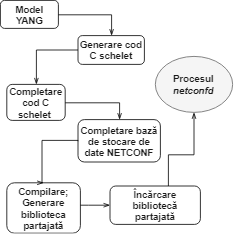
\includegraphics{dvm_v01_workflow}
	\caption{Organigramă a dezvoltării și implementării DVM \cite{stancu2016default}.}
	\label{fig:dvm_v01_workflow}
\end{figure}

Cel de-al doilea pas al implementării a constat în procesarea modelelor \gls{yang} alese și generarea codului C schelet al modulelor asociate acestora. Acest lucru a fost realizat cu utilitarul \textit{yangdump} oferit de soluţia \textit{OpenYuma}. Pentru a îmbunătăţi flexibilitatea \gls{dvm} și pentru a avea o mai bună separare între codul folosit de server și codul utilizatorului, care trebuie rescris, utilitarul a fost folosit cu opţiunea \textit{--split}. Astfel, pentru fiecare modul au fost generate patru fişiere: câte unul \textit{.c} și \textit{.h} pentru codul de server, respectiv pentru cel de utilizator.

Următorul pas a fost reprezentat de implementarea funcţiilor cu apel invers generate pentru fiecare atribut al modelului \gls{yang}. Pentru a asocia câte o valoare implicită fiecărui parametru, funcțiile au fost modificate astfel încât să întoarcă valoarea respectivă în momentul apelării.

Cea mai importantă parte a implementării \gls{dvm} a constat în construirea bazei de stocare a datelor de operare, reprezentând de fapt arborele atributelor \gls{yang} pe care serverul \gls{netconf} le va utiliza atunci când va fi interogat de către echipamentul de control \gls{sdn}. Nu a fost posibilă construirea automată a acestui arbore de parametri, astfel că atributele au fost implementate manual, de la rădăcină către frunze. Pentru acest lucru a fost nevoie să se altereze funcţia de iniţializare \textit{init2()} generată automat pentru fiecare model \gls{yang}. A fost necesară adăugarea câte unui nod \textit{OpenYuma} pentru fiecare parametru \gls{yang}, având asociată o funcție cu apel invers în care se setează valoarea implicită a acelui atribut. În cazul parametrilor anterior menţionaţi, care fac parte din fişierul de configurare, implementarea funcţiei constă în citirea valorii respective din acel fişier. Această abordare a permis utilizatorilor \gls{dvm} un acces facil la valorile implicite asociate fiecărui atribut. Dacă un utilizator avea nevoie de schimbarea valorii unui parametru \gls{yang}, o putea face uşor prin funcţia cu apel invers asociată sau prin fişierul de configurare, fără să fie nevoit să ştie detaliile de implementare referitoare la construirea arborelui de valori.

Următorii paşi ai implementării sunt simpli și direcţi: codul rezultat se compilează, rezultând bibliotecile partajate care apoi sunt încărcate în serverul \gls{netconf} (mai exact în procesul \textit{netconfd} asociat acestuia).

Etapele anterior menţionate se aplică în cazul modelului informațional de bază și în cazul modelului informațional pentru microunde, excluzând cazul notificărilor \gls{netconf}, unde abordarea este puţin diferită.

Deoarece modelul asociat notificărilor \gls{netconf}, \textit{MicrowaveModel-Notifications}, are o structură diferită, conţinând obiecte \gls{yang} ce reprezintă notificări în locul atributelor obişnuite, comportamentul soluţiei \textit{OpenYuma} este diferit în acest caz. În loc să se genereze funcții cu apel invers pentru obţinerea și setarea valorilor atributelor, în cazul notificărilor soluţia \textit{OpenYuma} va genera funcții cu apel invers folosite pentru declanşarea acestora (trimiterea lor de către server tuturor utilizatorilor care s-au abonat).

Pentru implementarea notificărilor \gls{netconf} în \gls{dvm}, un nou fir de execuţie s-a creat în funcţia de iniţializare a modulului, \textit{init2()}. Acesta rulează o singură funcție care implementează o buclă infinită în care se folosește funcţia cu apel invers asociată pentru a trimite o notificare fictivă, la un interval de secunde definit în fişierul de configurare. În cazul în care valoarea intervalului este zero, declanşarea notificărilor nu va fi activată. Detaliile conţinute în notificarea \gls{netconf} fictivă se găsesc în interiorul funcţiei care implementează generarea și modificarea acestora nu este banală pentru un utilizator neexperimentat.

Structura fişierului de configurare este foarte simplă și nu oferă prea multă flexibilitate utilizatorilor \gls{dvm}. Aceasta este fixă și poate fi observată în Figura \ref{fig:dvm_v01_config}, într-un exemplu în care un dispozitiv conţine două interfețe radio. Conţine doar trei tipuri de parametri, așa cum a fost menţionat anterior: numele echipamentului de rețea (\textit{NeName}), identificatoarele legăturilor radio (\textit{radioSignalId} - există câte un identificator pentru fiecare interfață radio a dispozitivului) și intervalul de timp, exprimat în secunde, dintre două notificări fictive consecutive (\textit{eventFrequency}).

\begin{figure}[h]
	\centering
	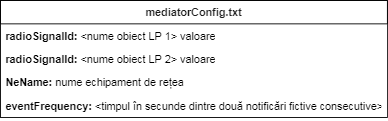
\includegraphics{dvm_v01_config}
	\caption{Structura fişierului de configurare al DVM. Exemplu pentru un echipament cu două interfețe radio.}
	\label{fig:dvm_v01_config}
\end{figure}
\section{Folosirea în contextul demonstraţiilor de concept a DVM versiunea 1}

Prima versiune a mediatorului cu valori implicite a fost o unealtă foarte importantă în contextul celei de-a doua demonstraţii de concept a proiectului rețelelor de transport de date fără fir din cadrul \gls{onf}. Acesta a ajutat la accelerarea implementării aplicațiilor \gls{sdn} care au fost dezvoltate pentru cazurile de utilizare propuse în \cite{onf2016_poc2}.

\gls{dvm} a oferit interfaţa de Sud \gls{netconf} care expune modelele informaționale dezvoltate de \gls{onf}, în același mod în care ar expune-o un mediator real ce se conectează la echipamente de transport de date fără fir. În acest mod, dezvoltatorii aplicațiilor \gls{sdn} au putut utiliza acest simulator pentru implementarea și testarea acestora, fără a avea nevoie să deţină dispozitive de rețea, care au un preţ foarte ridicat.

Această primă versiune de simulator a accelerat activitățile de pregătire a celei de-a doua demonstraţii de concept, permiţând lucrul în paralel la aplicațiile \gls{sdn} și la dezvoltarea mediatoarelor. Interfaţa \gls{netconf} comună a putut fi testată înainte ca producătorii de echipamente să își implementeze mediatoarele, oferind astfel mai mult timp dezvoltatorilor aplicațiilor \gls{sdn} pentru depanarea programelor. De exemplu, generarea unei notificări \gls{netconf} se poate face mult mai facil cu ajutorul simulatorului. Pentru un mediator real, trebuie ca dispozitivul să fie făcut să genereze o notificare către mediator, prin interfaţa proprietară echipamentului respectiv, apoi mediatorul să traducă acel mesaj într-o notificare \gls{netconf}.

Figura \ref{fig:dvmv01_poc_usage} reprezintă elementele de bază ale demonstraţiei de concept, așa cum sunt prezentate în lucrarea apărută după desfăşurarea acestuia \cite{onf2016_poc2}, în care se poate vedea \gls{dvm}.

\begin{figure}[h]
	\centering
	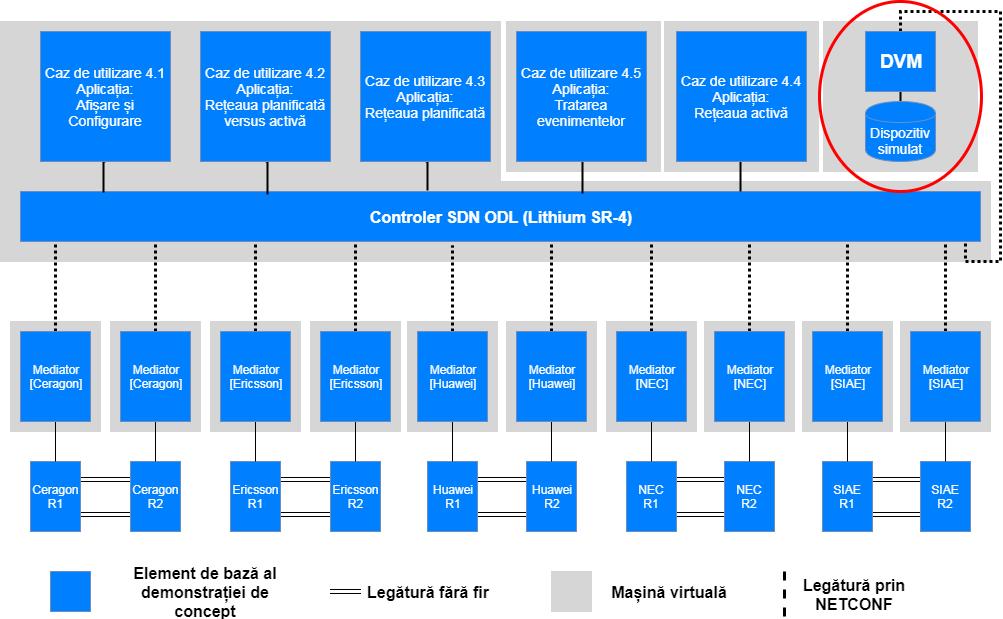
\includegraphics[width=1\textwidth]{dvmv01_poc_usage}
	\caption{Configurarea rețelei de test SDN utilizând mașini virtuale \cite{onf2016_poc2}.}
	\label{fig:dvmv01_poc_usage}
\end{figure}

Înregistrarea la controlerul \gls{sdn} a primei versiuni a simulatoarelor \gls{dvm}, se face la fel ca pentru un mediator real. Astfel, echipamentul de control oferă o interfață de programare a aplicaţiei - \gls{api} - prin care o aplicație \gls{sdn} poate înregistra un astfel de mediator în controlerul \gls{sdn}. Înregistrarea nu este una automată, utilizatorul fiind nevoit să facă această înregistrare manual. În cea de-a doua demonstraţie de concept, acest lucru a fost făcut prin interfaţa grafică a echipamentului de control folosit (\gls{odl}). După înregistrare, controlerul stabileşte conexiunea \gls{netconf} cu mediatorul.

Codul asociat primei versiuni a \gls{dvm} este oferit cu sursă deschisă și se poate găsi în repertoriul asociat \gls{onf} de pe platforma GitHub, denumit CENTENNIAL \cite{dvmv01github}.
\section{Arhitectura DVM versiunea 2}

Cea de-a doua versiune a \gls{dvm} a fost implementată pentru a treia demonstraţie de concept a rețelelor de transport de date fără fir desfăşurată în cadrul \gls{onf}. A fost dezvoltată pe scheletul primei versiuni, păstrând aceeaşi abordare: un server \gls{netconf} care se bazează pe soluţia software \textit{OpenYuma} și un fişier de configurare din care serverul poate citi valori pentru atributele \gls{yang} pe care le expune. Din acest punct de vedere, \gls{dvm} versiunea 2 folosește întregul model informațional pentru microunde TR-532 și o parte semnificativă din modelul informațional de bază, TR-512.1, cumulând aproximativ 300 de astfel de parametri.

Arhitectura celei de-a doua versiuni a \gls{dvm} este influenţată de natura atributelor \gls{yang} ce alcătuiesc modelul informațional pentru microunde \cite{stancu2017enabling}: parametri de configurare, de stare sau care prezintă capabilitățile dispozitivului. Atributele de configurare pot fi citite sau scrise și prin intermediul acestora un utilizator poate influenţa comportamentul dispozitivului. Parametrii de stare pot fi doar citiţi și reprezintă situația curentă a echipamentului, în timp ce capabilitățile sunt atribute care pot fi doar citite și descriu abilităţile dispozitivului.

Mediatorul cu valori implicite a fost gândit astfel încât să fie flexibil și să ofere posibilitatea înlocuirii citirii valorilor din fişierul de configurare cu o citire dintr-un echipament real, cu ajutorul unui protocol la alegere. Deoarece mediatorul este o aplicație software externă, care nu face parte din echipamentele de transport de date fără fir, în momentul inițializării ar trebui să reflecte configurația echipamentului la care se conectează. Din cauza faptului că dispozitivul nu are o configuraţie statică și aceasta poate fi modificată înaintea inițializării mediatorului, nu poate fi utilizată baza de stocare de date de iniţializare oferită de serverul \gls{netconf}. Asta înseamnă ca în momentul inițializării mediatorul trebuie să își construiască baza de stocare de date de operare într-un mod arborescent, interogând dispozitivul de rețea asupra valorilor atributelor. Acest lucru se aplică doar în cazul parametrilor configurabili sau în cazul celor care au un caracter static, precum capabilitățile echipamentului. Deoarece aceste valori se salvează în baza de stocare de date de operare, înseamnă că acestea nu sunt persistente și vor fi citite la fiecare iniţializare din dispozitiv. Fiindcă simulatorul \gls{dvm} a fost proiectat ca un mediator real, toate aceste aspecte se reflectă și în arhitectura acestuia, diferenţa fiind că valorile atributelor nu se citesc dintr-un dispozitiv, ci dintr-un fişier de configurare descris în limbajul \gls{xml}.

Natura atributelor \gls{yang}, descrisă anterior, a dus la arhitectura celei de-a doua versiuni a \gls{dvm} care se poate vedea în Figura \ref{fig:dvm_v02_architecture}. Atributele \gls{yang} au fost împărţite în trei categorii: de iniţializare, de execuţie și de configurare.

\begin{figure}[h]
	\centering
	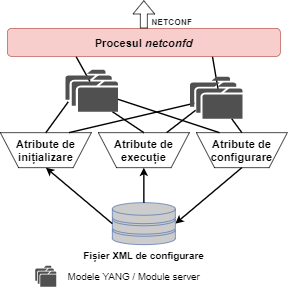
\includegraphics{dvm_v02_architecture}
	\caption{Arhitectura simulatorului DVM versiunea 2.}
	\label{fig:dvm_v02_architecture}
\end{figure}

Parametrii de iniţializare reprezintă acele atribute statice, care sunt citite din dispozitiv o singură dată, în momentul inițializării simulatorului. În cadrul serverului \gls{netconf} pot fi doar citite, în cazul parametrilor care reprezintă capabilitățile echipamentului (adică informaţie statică, prezentată de către dispozitiv, care nu se poate schimba) sau pot fi și scrise și citite, ca în cazul parametrilor de configurare. În momentul inițializării \gls{dvm} aceștia sunt consideraţi parametri de iniţializare, ca apoi să devină de configurare, având câte o funcție cu apel invers asociată, care permite modificarea acestei valori în fişierul \gls{xml} de configurare prin intermediul serverului \gls{netconf}. Nu este nevoie ca aceste atribute de configurare să fie citite din dispozitiv decât în momentul inițializării, deoarece apoi se presupune că orice configurare asupra dispozitivului se va face prin echipamentul de control \gls{sdn}, deci prin intermediul serverului \gls{netconf} care va fi astfel informat asupra noii valori a parametrilor respectivi.

Atributele de execuţie reprezintă parametrii dinamici, care pot fi doar citiţi ai dispozitivului, precum alarme, informații de stare sau de monitorizare a performanţelor. Acestea trebuie citite din echipament de fiecare dată când controlerul \gls{sdn} le cere, din cauza naturii lor dinamice. Soluția acestei abordări constă în nodurile virtuale oferite de soluția \textit{OpenYuma}. În loc de a avea o valoare stocată pentru un atribut \gls{yang}, sau valori pentru grupuri de atribute, \textit{OpenYuma} oferă posibilitatea de a asocia o funcție cu apel invers pentru astfel de parametri. Aceasta va fi apelată de fiecare dată când valoarea atributului asociat este cerută serverului \gls{netconf}, iar implementarea acesteia va prelua valoarea din fişierul \gls{xml} de configurare, sau va construi arborele asociat răspunsului, în cazul unui grup de atribute.

Cea de-a doua versiune a simulatorului \gls{dvm} se bazează pe abordarea \textit{OpenYuma} de a folosi funcții cu apel invers pentru implementarea funcţionalităţii de citire sau scriere asociată atributelor modelelor \gls{yang}. Proiectarea \gls{dvm} urmăreşte separarea descrisă anterior a parametrilor, oferind diferite funcții cu apel invers pentru diferitele categorii. Fiecare atribut din modelele \gls{yang} va fi modelat ca un nod \textit{OpenYuma}, care reprezintă un tip de date pus la dispoziţie de această soluție software, conţinând diverse informații rezultate din analizarea modelului \gls{yang}, precum numele, constrângeri asupra valorilor pe care atributul le poate lua și funcţia cu apel invers asociată, de citire sau de scriere. Astfel, au fost considerate trei funcții cu apel invers generice, care să fie folosite în cele trei cazuri date de împărțirea atributelor \gls{yang}: pentru parametrii de iniţializare, de execuţie și de configurare. Acestea sunt considerate generice, deoarece o singură astfel de funcție cu apel invers este utilizată pentru fiecare tip de atribut, diferenţierea pentru fiecare atribut în parte făcându-se în implementarea acesteia, în funcție de numele atributului. Această abordare oferă flexibilitate și uşurinţă în implementarea simulatorului \gls{dvm}.


\section{Implementarea DVM versiunea 2}

Istoria reţelelor definite prin software.
\section{Folosirea în contextul demonstraţiilor de concept a DVM versiunea 2}

Așa cum prima versiune a \gls{dvm} a fost foarte importantă în contextul celei de-a doua demonstraţii de concept a rețelelor de transport de date fără fir și a doua versiune a acestui simulator a fost o unealtă critică pentru pregătirea celei de-a treia demonstraţii de concept. A permis dezvoltatorilor de aplicații \gls{sdn} să le testeze și să le depaneze într-o manieră facilă, eliminând necesitatea deţinerii unor echipamente de rețea și a mediatorului asociat.

\gls{sdn} nu influenţează doar modul în care rețelele sunt controlate și administrate, ci și modul în care sunt organizate proiectele și modul în care anumite cerinţe și capabilităţi sunt dezvoltate și implementate. Dacă înainte aplicațiile și dispozitivele de rețea erau oferite împreună, de către producătorii de echipamente, interfeţele standard dintre dispozitive și echipamentele de control \gls{sdn}, sau dintre echipamentele de control și aplicații, oferă posibilitatea companiilor de a oferi doar anumite secţiuni din întreaga soluție. Aceste companii pot profita de simulatorul \gls{dvm}, deoarece le oferă acces la aceste interfețe fără a avea nevoie să deţină echipamente de rețea foarte scumpe.

Avantajul pe care \gls{dvm} îl oferă și care a fost folosit în cea de-a treia demonstraţie de concept \gls{onf} este reprezentat de faptul că orice modificare în modelele \gls{yang} dezvoltate poate fi testată cu ajutorul simulatorului, deoarece acesta oferă o modalitate rapidă de a o implementa, simulând astfel, din punctul de vedere al echipamentului de control \gls{sdn}, interacţiunea cu un dispozitiv de rețea. După dezvoltarea simulatorului și a aplicațiilor \gls{sdn}, acestea din urmă pot fi testate, chiar înainte ca software-ul din elementele de rețea să fie implementat. Cu toate acestea, este nevoie ca aplicațiile să efectueze teste de integrare cu dispozitivele de rețea, deoarece comportamentul simulatorului nu poate fi identic cu cel al echipamentelor. Simulatorul \gls{dvm} folosit în cea de-a treia demonstraţie de concept nu a simulat dispozitivele de rețea, ci nivelul mediator care oferă interfaţa \gls{netconf} ce expune modelele \gls{yang} dorite. A fost posibilă simularea diferitor topologii de rețea, având dispozitive cu diferite configurări și interfețe de transport de date. Simulatorul \gls{dvm} a fost și în cazul celor de-a doua și de-a treia demonstraţii de concept \gls{onf} unealta principală pentru a putea crea o topologie de rețea simulată \cite{onf2016_poc2, onf2016_poc3}. 

Simulatorul a fost folosit și pentru teste de extensibilitate și de performanţă ale aplicațiilor \gls{sdn} dezvoltate. Fişierul \gls{xml} de configurare poate fi manipulat foarte uşor, adăugând interfețe de transport de date echipamentelor sau intrări pentru valorile indicatorilor de performanţă. De exemplu, un dispozitiv de rețea are nevoie de 24 de ore pentru a genera 96 de intrări ale indicatorilor de performanţă de 15 minute și 30 de zile pentru a genera 30 de intrări ale indicatorilor de performanţă de 24 de ore. O altă funcție importantă a \gls{dvm} care a fost folosită în pregătirea demonstraţiei de concept a fost cea de generare a notificărilor \gls{netconf}. Au putut fi simulate diferite tipuri de notificări care să apară la un interval de timp configurabil.

În mod evident, timpii de răspuns ai simulatorului sunt foarte reduşi, deoarece nu există o comunicaţie cu un echipament de rețea real, deci nici nevoia de a procesa valorile atributelor care sunt citite din dispozitivele de rețea. Nevoia de a procesa valorile unor atribute apare în cazul mediatoarelor reale, în momentul în care atributele definite în modelul informațional pentru microunde nu se potrivesc în totalitate cu atributele dispozitivului și o anume procesare a acelei valori este necesară pentru a transforma-o în ce se doreşte în modelul \gls{yang}.

Tabelul \ref{tab:Table_3} ilustrează diferenţele între \gls{dvm} și un mediator real, în diferite situaţii care au apărut în pregătirea celei de-a treia demonstraţii de concept \gls{onf} \cite{stancu2017enabling}.

\begin{table}[h]
	
	\caption{Comparaţie între comportamentele unui mediator real și al simulatorului în diferite situații \cite{stancu2017enabling}.\label{tab:Table_3}}
	\begin{tabular}{|M{0.5\textwidth}|M{0.2\textwidth}|M{0.2\textwidth}|}
		\hline
		\textbf{Situația} & \textbf{\emph{Mediator real}} & \textbf{\emph{Simulatorul DVM}} \tabularnewline
		\hline 
		Dezvoltarea aplicațiilor \gls{sdn} & costisitoare & eficientă \tabularnewline
		\hline 
		Timpul de implementare & greoi & rapid \tabularnewline
		\hline 
		Topologia de rețea & complex de schimbat & flexibilă, uşor de schimbat \tabularnewline
		\hline 
		Generarea notificărilor \gls{netconf} & greu de controlat & simplă \tabularnewline
		\hline 
		Timpi de răspuns & reali & nerealişti \tabularnewline
		\hline 
		Procesare a valorilor atributelor & în unele cazuri & nu este nevoie \tabularnewline
		\hline \end{tabular}
\end{table}

Pentru a oferi un suport mai bun testelor de extensibilitate și de performanţă ale aplicațiilor, simulatorul \gls{dvm} ar fi putut implementa timpi de răspuns configurabili la operaţiile \gls{netconf} sau generarea de notificări care să urmărească anumite pofile temporale, în funcție de nevoile aplicațiilor \gls{sdn}.

La fel ca în cazul versiunii anterioare a \gls{dvm}, înregistrarea simulatoarelor la echipamentul de control \gls{sdn} se face manual, cu ajutorul interfeţei grafice a controlerului, care stabileşte apoi conexiunea securizată și iniţiază o sesiune \gls{netconf}.
\section{Integrarea DVM cu comutatorul software LINC: \textit{LINC-WE}}

Așa cum a fost descris anterior, simulatorul \gls{dvm} permite emularea nivelului mediator care apare în arhitectura \gls{sdn} a rețelelor de transport de date fără fir. Se pot simula diferite topologii de rețea prin manipularea fişierelor \gls{xml} de configurare ale diferitelor instanţe ale \gls{dvm}, făcând simulatoarele să prezinte diferite configuraţii. Această abordare oferă un bun prim pas pentru simularea rețelelor de transport de date fără fir în contextul \gls{sdn}, însă nu este suficient, deoarece instanţele \gls{dvm} sunt independente și rețeaua simulată nu este completă. În plus, nu există legături între dispozitivele simulate. Din acest motiv, această secţiune prezintă încercarea de a integra simulatorul \gls{dvm} cu un comutator software deja existent, care a fost folosit anterior pentru simulări de rețele optice în contextul \gls{sdn}: \textit{Legătura Nu Este Închisă} - \gls{linc} și cu simulatorul de rețele definite prin software, \textit{mininet}. Comutatorul software folosit anterior în simularea rețelelor optice~\cite{parulkar2015sdn, kretsis2016emulation, mehmeri2017software}, bazat pe \gls{linc} se numeşte \textit{Legătura Nu Este Închisă - Extensii Optice} - \gls{linc-oe}, astfel că am denumit comutatorul rezultat în urma integrării \gls{dvm} cu \gls{linc}: \textit{Legătura Nu Este Închisă - Emulator Fără Fir} - \gls{linc-we}~\cite{stancu2017wireless}.

\subsection{LINC}

\gls{linc} este un comutator software ce suportă protocolul OpenFlow, scris în limbajul de programare Erlang~\cite{lincsw}. Acesta a fost proiectat să fie modular, oferind o metodă rapidă de a face prototipuri \gls{sdn} și de a testa noi caracteristici ale protocolului OpenFlow. Este oferit ca o implementare cu sursă deschisă de către \textit{FlowForwarding.org} și are ca scop oferirea unei soluții prin care utilizatorii pot evalua rapid protocoalele OpenFlow și OF-Config.

Un singur comutator este implementat ca un nod Erlang și cuprinde mai multe comutatoare logice. Acestea, porturile și legăturile dintre porturi sunt descrise de către utilizator prin intermediul unui fișier de configurare, așa cum este ilustrat și în Figura \ref{fig:linc_architecture}. Datorită acestei arhitecturi modulare, comutatorul \gls{linc} este capabil să ofere mai multe implementări pe care utilizatorul le poate alege, fiecare având asociată o versiune diferită a protocolului OpenFlow (versiunile 1.2, 1.3 sau 1.4). Aceste implementări sunt responsabile de comutarea pachetelor și modificarea tabelelor de fluxuri de date.

\begin{figure}[h]
	\centering
	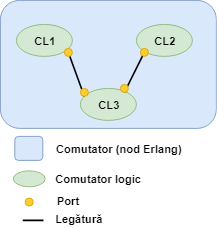
\includegraphics{linc_architecture}
	\caption{Arhitectura comutatorului software LINC~\cite{linc2014qsg}.}
	\label{fig:linc_architecture}
\end{figure}

După cum este prezentat în~\cite{linc2014qsg}, \gls{linc} prezintă mai multe blocuri software: comutatorul capabil OpenFlow, modului protocolului OpenFlow, modului protocolului OF-Config. Acestea sunt dezvoltate ca aplicații Erlang separate, respectând principiile \textit{Platforma Telecom Deschisă} - \gls{otp} ale limbajului Erlang. Există și o componentă separată care se ocupă de conexiunea la un echipament de control \gls{sdn}. Tabelele de fluxuri, porturile sau tabelele de grup sunt administrate de implementările separate reprezentând diferitele versiuni ale protocolului OpenFlow.

\subsubsection{LINC-OE}

Datorită naturii modulare a comutatorului \gls{linc}, a apărut o nouă implementare care să acopere cazurile de utilizare ale \gls{sdn} din domeniul optic: \gls{linc-oe} \cite{parulkar2015sdn}. Acesta reprezintă un simulator de comutatoare optice care suportă extensiile optice ale protocolului OpenFlow. Diferenţa dintre \gls{linc} și \gls{linc-oe} este că, în cazul celui din urmă, comutatoarele logice care sunt simulate reprezintă comutatoare optice, astfel încât spre deosebire de interfeţele electrice, porturile optice oferă mai multe canale de comunicaţie independente, diferenţiate prin lungimea de undă. În implementarea \gls{linc-oe}, mesajele ce se transmit printr-un astfel de port optic nu mai sunt pachete Ethernet, ci mesaje Erlang, ce conţin informații adiţionale, pe lângă pachetul Ethernet propriu-zis. O altă diferenţă este dată de faptul ca \gls{linc-oe} oferă interfețe pentru simularea defectării legăturilor dintre porturi.

\subsubsection{Interfaţa NETCONF}

Comutatorul software \gls{linc} include de asemenea și o interfață \gls{netconf}. Este folosită de către protocolul OF-Config și este disponibilă pentru un comutator doar dacă acel protocol este folosit. În cazul în care este permisă utilizarea acestuia, o nouă aplicație Erlang este pornită în cadrul nodului Erlang: \textit{enetconf}, care pornește un server \gls{netconf} ce aşteaptă conexiuni pe adresa \gls{ip} și portul selectate de utilizator.

Această abordare prezintă un dezavantaj major: doar un singur server \gls{netconf} este pornit pentru comutatorul \gls{linc}, astfel că nu se pot accesa comutatoarele logice care alcătuiesc comutatorul \gls{linc} individual prin interfaţa \gls{netconf}. Acestea pot fi configurate doar prin intermediul protocolului OpenFlow \cite{lincsw}.

De asemenea, modelul informațional \gls{yang} care este oferit de către server nu este configurabil, astfel încât utilizatorul nu poate alege un model \gls{yang} pe care comutatorul software să îl poată folosi. Dacă acest lucru ar fi fost oferit, ar fi fost banală transformarea \gls{linc-oe} în \gls{linc-we}, prin înlocuirea modelului \gls{yang} expus cu modelul informațional pentru microunde și apoi corelarea atributelor \gls{yang} cu parametrii comutatorului \gls{linc}.

\subsection{LINC-WE}

\gls{linc-we} a apărut ca o încercare de a îmbunătăţi simulatorul \gls{dvm} dezvoltat anterior, prin oferirea unei soluții care să simuleze nu doar dispozitive de rețea independente, ci și legăturile dintre acestea. Astfel, am luat în considerare integrarea \gls{dvm} cu un comutator software deja existent, \gls{linc}, având în vedere și faptul că acesta a fost folosit anterior pentru simularea de rețele optice în contextul \gls{sdn}, prin \gls{linc-oe} \cite{parulkar2015sdn}.

Spre deosebire de \gls{linc} și \gls{linc-oe}, \gls{linc-we} nu ilustrează utilizarea protocolului OpenFlow pentru configurarea comutatorului, ci pune accent pe protocolul \gls{netconf} pentru administrarea dispozitivelor de rețea. Oferă totuşi suportul pentru protocolul OpenFlow, prin modulele \gls{linc} care implementează versiunile 1.2, 1.3 și 1.4 ale acestuia. Deoarece configurarea și administrarea dispozitivelor de transport de date fără fir a migrat de la protocolul OpenFlow (prin dezvoltarea de extensii specifice) la \gls{netconf}, așa cum demonstrează activitatea de cercetare din cadrul \gls{onf}, prin apariția modelelor informaționale care pot fi ușor transformate în modele \gls{yang} \cite{onftr532, onftr512v1.0, onftr512v1.1, onftr512v1.2}, această abordare oferind mai multă flexibilitate. \gls{linc-we} încearcă să construiască pe această bază prin oferirea unui comutator software care să expune modelele \gls{yang} propuse de \gls{onf} și să poată fi folosit în simulări.

Abordarea aleasă în acest caz a fost înlocuirea aplicaţiei Erlang \textit{enetconf}, care implementa serverul \gls{netconf} pentru comutatorul software \gls{linc} cu o aplicație externă, dezvoltată în C, care să expună modelele \gls{yang} specifice rețelelor de transport de date fără fir: \gls{dvm}.

Implementarea serverului \gls{netconf} este dată de simulatorul descris anterior, \gls{dvm}. Pentru integrarea acestuia cu comutatorul software \gls{linc} am înlocuit aplicaţia Erlang ce implementa suportul pentru acest protocol, \textit{enetconf}, cu o aplicație Erlang nouă, dezvoltată în acest scop: \textit{erl\_yuma}. Aceasta se ocupă de pornirea și oprirea serverului \gls{netconf} implementat pentru \gls{dvm}, prin deschiderea unui port Erlang care va avea această sarcină. Codul acestei soluții este oferit cu sursă deschisă și poate fi găsit pe platforma GitHub~\cite{lincwe2017}.

Din punctul de vedere al echipamentului de control \gls{sdn}, acesta va comunica prin interfaţa \gls{netconf} cu \gls{dvm}, care a fost pornit anterior din mediul Erlang (prin aplicaţia \textit{erl\_yuma}). Comunicaţia dintre aplicațiile dezvoltate în Erlang și în C este administrată de către sistemul de execuţie Erlang. Din perspectiva \textit{erl\_yuma}, comunicaţia cu \gls{dvm} se face prin mesaje standard Erlang, care sunt transmise prin portul Erlang asociat acesteia. Din cealaltă perspectivă, a \gls{dvm}, comunicaţia se realizează prin fluxurile standard de intrare și de ieșire, \textit{stdin} și \textit{stdout}. O imagine de ansamblu a arhitecturii \gls{linc-we} este prezentată în Figura \ref{fig:linc_we_architecture}.

\begin{figure}[h]
	\centering
	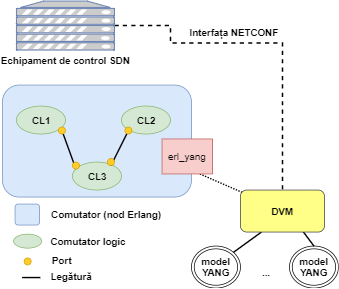
\includegraphics{linc_we_architecture}
	\caption{Arhitectura comutatorului software LINC-WE~\cite{linc2014qsg}.}
	\label{fig:linc_we_architecture}
\end{figure}

Restul arhitecturii \gls{linc} nu este influenţată: există în continuare comutatorul software, care expune o interfață \gls{netconf} (doar că acum este oferită prin \gls{dvm}) și conţine mai multe comutatoare logice, împreună cu porturile acestora și legăturile dintre ele, așa cum a fost definit în fişierul de configurare \gls{linc}. Aplicaţia ce oferă interfaţa \gls{netconf}, \textit{erl\_yuma}, este pornită doar în cazul în care protocolul OF-Config este activat.

\subsubsection{Interfața NETCONF - Aplicația Erlang}

Aplicaţia care transformă comutatorul software \gls{linc} în \gls{linc-we}, prin integrarea cu \gls{dvm} este \textit{erl\_yuma}. Aceasta este o aplicație Erlang tipică, ce respectă principiile \gls{otp} \cite{logan2010erlang}.

Structura aplicaţiei respectă recomandările \gls{otp}. În dosarul rădăcină \textit{erl\_yuma} al aplicaţiei sunt create următoarele directoare: \textit{ebin}, ce conţine fişierele compilate *.beam, dar și fişierul de resurse ale aplicaţiei \gls{otp} (ce conţine informații precum descrierea, versiunea, etc.). Directoarele \textit{include} și \textit{priv} ar trebui să conţină fişierele de incluziune *.hrl și respectiv aplicațiile externe de care depinde aplicaţia Erlang. Încă două dosare alcătuiesc aplicaţia: \textit{src}, unde se găsesc fişierele sursă și \textit{test}, ce conţine fişiere de test.

O imagine de ansamblu a aplicaţiei Erlang poate fi văzută în Figura \ref{fig:erlang_application}. Există trei fişiere sursă importante: \textit{ey\_app.erl}, \textit{ey\_sup.erl} și \textit{ey\_server.erl}.

\begin{figure}[h]
	\centering
	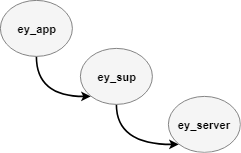
\includegraphics{erlang_application}
	\caption{Structura aplicației Erlang \textit{erl\_yuma}~\cite{linc2014qsg}.}
	\label{fig:erlang_application}
\end{figure}

Primul fişier sursă, \textit{ey\_app.erl}, reprezintă implementarea unui comportament \textit{aplicație}, așa cum este definit în \gls{otp}. Este o implementare simplă și directă a acestui comportament \gls{otp}, care oferă doar două funcții cu apel invers: \textit{start} și \textit{stop}. Prima este folosită pentru a porni procesul care este responsabil pentru implementarea aplicaţiei. Acesta este un proces \gls{otp} supervizor.

Cel de-al doilea fişier sursă, \textit{ey\_sup.erl}, implementează un comportament \textit{supervizor} definit de \gls{otp}. Acesta este procesul central al aplicaţiei \textit{erl\_yuma} și este responsabil pentru supravegherea acestuia. Este necesară implementarea unei singure funcții cu apel invers oferite de acest comportament: \textit{init}. În momentul în care procesul supervizor este pornit, această funcție este invocată, acesta fiind și locul în care ar trebui să pornim procesul \textit{ey\_server.erl}, conform cu structura aplicaţiei noaste. Nu trebuie să pornim mai multe procese copil în acest punct, deoarece dorim să expunem o singură interfață \gls{netconf}. Astfel, procesul supervizor va porni un singur modul \textit{ey\_server}.

Ultimul fişier sursă care alcătuieşte aplicaţia \textit{erl\_yuma} este \textit{ey\_server.erl}. Din punctul de vedere \gls{otp}, acest modul implementează un comportament \textit{gen\_server} (server generic). Acest proces este responsabil de crearea unui port Erlang, care porneşte aplicaţia externă C, reprezentată de \gls{dvm}. Astfel, procesul va stoca portul care a fost creat. În funcţia cu apel invers \textit{init}, practic însemnând atunci când procesul este pornit, un port Erlang este creat. Intern, acest lucru înseamnă crearea unui nou proces, bazată pe o anumită comandă. Comanda este definită ca o variabilă de mediu și este stocată în fişierul de resurse ale aplicaţiei și reprezintă de fapt comanda necesară pornirii \gls{dvm}. A fost folosită această abordare pentru a fi uşor de modificat în cazul în care comanda cu care se porneşte \gls{dvm} se va schimba pe viitor. Astfel, aplicaţia Erlang nu va trebui recompilată.

Un aspect interesant îl constituie modalitatea în care portul Erlang trebuie închis. Când utilizatorul doreşte închiderea \gls{linc-we}, trebuie ca și \gls{dvm} să fie închis, astfel încât să fie pregătit pentru o eventuală viitoare rulare. Acest lucru se face prin implementarea funcţiei cu apel invers \textit{terminate} a modulului \textit{ey\_server}. Este important de menţionat faptul că pentru ca această funcție să fie invocată în momentul închiderii aplicaţiei, aceasta trebuie să proceseze mesaje capcană (\textit{trap message}). Implementarea funcţiei \textit{terminate} va trebui să închidă instanţa \gls{dvm} care rulează (prin trimiterea unui semnal de închidere a procesului către sistemul de operare).

În prima versiune a \gls{linc-we} nu a fost implementată comunicaţia dintre aplicațiile Erlang și C. Cu ajutorul acesteia s-ar fi putut manipula parametrii comutatorului software, prin operații \gls{netconf}. Practic, \gls{linc-we} doar crează o instanţă un simulator \gls{dvm}, expunând o interfață \gls{netconf}, care însă nu implementează și modificarea atributelor comutatorului \gls{linc}.

\subsection{Concluziile integrării}

O unealtă ce oferă posibilitatea de a simula rețele ce conţin dispozitive de transport de date fără fir, care să expună și modelul informațional pentru microunde propus de \gls{onf} este importantă atât pentru membrii \gls{onf}, care pot testa, revizui și îmbunătăţi modelul, cât și pentru dezvoltatorii de aplicații \gls{sdn} care pot începe implementarea și testarea de software pentru astfel de rețele. Deoarece TR-532 a fost propus de curând, în decembrie 2016, nu există încă suport pentru acesta în simulatoare de rețea consacrate, precum OPNET sau OMNeT++, făcând \gls{linc-we} prima încercare de simulator care să ofere o astfel de interfață unui echipament de control \gls{sdn}.

\gls{linc-we} oferă posibilitatea unei lansări rapide a unui simulator ce suportă modelul TR-532 și, spre deosebire de \gls{dvm}, care era oferea doar serverul \gls{netconf} ce expunea modelele informaționale \gls{onf}, oferă și posibilitatea de a transmite trafic de date prin rețeaua simulată. Acest lucru este posibil deoarece \gls{linc-we} se bazează pe soluţia deja existentă și folosită în rețele optice, \gls{linc-oe}. Parte din cercetarea anterioară a fost și integrarea \gls{linc-oe} cu simulatorul de rețele definite prin software, \textit{mininet}, astfel că și \gls{linc-we} va fi integrat implicit cu această unealtă.

Această abordare a permis o integrare rapidă a \gls{linc} cu \gls{dvm}. După parcurgerea etapei destul de greoaie de învăţare a limbajului de programare Erlang, în care este implementat comutatorul software \gls{linc}, integrarea cu \gls{dvm} a fost facilă, aplicaţia Erlang ce se ocupă de acest aspect, descrisă anterior, fiind destul de simplă. Aceasta respectă principiile \gls{otp} și porneşte instanţa \gls{dvm} ce expune modelele \gls{yang} dorite.

Un alt avantaj oferit de această soluție este faptul că \gls{linc-we} oferă atât suport pentru protocolul \gls{netconf}, cât și pentru protocolul OpenFlow. Astfel, un echipament de control \gls{sdn} poate folosi, pe de o parte, interfaţa \gls{netconf} pentru a configura parametrii dispozitivelor simulate și, pe de altă parte, interfaţa OpenFlow pentru a administra traficul din rețea prin manipularea tabelelor de fluxuri ale echipamentelor.

Principalul dezavantaj al abordării folosite în cadrul \gls{linc-we} este faptul că poate oferi o singură interfață \gls{netconf}, care este asociată cu comutatorul software și nu câte o interfață \gls{netconf} pentru fiecare comutator logic din interiorul topologiei. Soluția evidentă ar fi pornirea câte unei aplicații \textit{erl\_yuma} pentru fiecare astfel de comutator, însă aceasta nu este banală și uşor de implementat, deoarece \gls{dvm} nu este proiectat să ruleze mai multe instanţe pe aceeaşi mașină, având anumite lucruri ce nu pot fi împărţite (de exemplu portul pe care aşteaptă conexiuni serverul \gls{netconf}, sau fişierul \gls{xml} de configurare).

Un alt dezavantaj îl constituie faptul că \gls{linc-we} nu este uşor de utilizat. Trebuie urmaţi mai mulți paşi înainte ca acesta să poată fi pornit: instalarea comutatorului software \gls{linc}, care implică instalarea mediului Erlang în prealabil; apoi, simulatorul \gls{dvm} trebuie instalat, după ce a fost instalată anterior soluţia software OpenYuma.

Fiind doar prima versiune a \gls{linc-we}, a fost implementată rapid pentru a putea fi folosită pentru teste. Asta înseamnă că se pot aduce multe îmbunătăţiri acestei soluții. Un aspect important ce ar putea fi luat în considerare este asocierea parametrilor din modelul informațional pentru microunde cu parametri reali din comutatorul software. Asta implică, însă, o înţelegere mai aprofundată a limbajului de programare Erlang. Implementarea comutatorului \gls{linc} ar putea ţine cont de aceşti parametri în simulare. De exemplu, dacă frecvenţele emiţătoarelor și receptoarelor unor porturi care comunică nu se potrivesc, comunicarea între acestea ar putea fi oprită în implementarea comutatorului.

Dată fiind dificultatea limbajului de programare Erlang și limitările descrise anterior, am renunţat la dezvoltarea unei a doua versiuni a \gls{linc-we} și am căutat o alternativă la această abordare care să fie mai facilă și mai uşor de dezvoltat și implementat. Soluția găsită a fost folosirea unei unelte de creare a unor containere software care pot rula într-un mod izolat anumite aplicații: \textit{docker}. Aceasta va fi detaliată în capitolul următor.